\documentclass{scrartcl}

\usepackage{graphicx}
\usepackage[utf8]{inputenc}
\usepackage[ngerman]{babel}
\RequirePackage[babel=true]{csquotes}
\defineshorthand{"`}{\openautoquote}
\defineshorthand{"'}{\closeautoquote}

\title{Einführung in LAFIC}
\title{Einführung in LAFIC}
\author{Sebastian Meisel}

\begin{document}

\maketitle


LAFIC bedeutet \textit{layout and format in comments}, also "`Layout
und Format in Kommentaren"', denn sämtliche Formatierungen
werden in LAFIC in Kommentarzeilen ausgeführt.

\section{Zeilen und Absätze}

Der Inhalt wird durch die Unterscheidung von  \emph{Zeilen} und
\emph{Absätze}n gegliedert.

Dabei besteht der Unterschied nicht so sehr in der
Länge. Vielmehr unterscheiden sich Zeilen von Absätze
dadurch, dass sie kein Satzschlusszeichen (., ?, !, :).
Wenn nicht anders festgelegt, werden sie als Überschriften
interpretiert.

Die erste \emph{Zeile} wird als Titel interpretiert und zu \textbackslash title
umgewandelt, wenn die Datei in LaTeX umgewandelt wird, bei
HTML-Ausgabe wird es in <h1> umgewandelt.

Weitere \emph{Zeilen} werden in <h3> (\textsc{HTML}) oder \textbackslash section
(LaTeX) umgewandelt, wenn es nicht anders angegeben wird.

Auf diese Weise können einfache Texte ganz ohne Formatierung
gegliedert werden.

\section{Kommentare}

Man kann im Text jeder Zeit Kommentare einführen in dem man einen Absatz einfügt, der mit zwei \%-Zeichen beginnt:

\begin{quote}
  \%\% Dies ist ein Kommentar.

  \%\% Dies ist ein längerer Kommentar. Es ist wichtig, dass
  \%\% Kommentare immer durch eine Leerzeile vom eigentlichen
  \%\% Inhalt getrennt sind.

\end{quote}



\section{Formatierte Absätze}

Absätze können formatiert werden, in dem eine Zeile
vorangestellt wird, die mit einem \%-Zeichen beginnt dem ein
Schlüsselwort folgt. Ist das Schlüsselwort bekannt, wird
die entsprechende Umgebung (LaTeX), bzw. der entsprechende
Block (Html) ausgegeben. Ansonsten dient das Schlüsselwort
(umgewandelt in Kleinschreibung) als Name der Umgebung
(LaTeX), bzw. eines <div>-Blocks (Html).

\begin{quote}
	\% Z
	Dieser Absatz ist zentriert.

\end{quote}

\begin{center}
Dieser Absatz ist zentriert.

\end{center}

Folgen zwei Absätze mit dem selben Schlüsselwort
hintereinander, werden sie in einer Umgebung / einem Block
zusammengefasst.

\begin{quote}
  \% Zitat\\
  Dies ist ein Zitat.\\

  \% Zitat\\
  Hier geht das Zitat weiter.\\

\end{quote}

Wird zu:

\begin{quote}
Dies ist ein Zitat.

Hier geht das Zitat weiter.

\end{quote}

Zur Zeit werden folgende Schlüsselworte unterstützt:

\begin{itemize}

\item Zitat für quote-Umgebung / <blockquote>-Block.
\item Langzitat / LZitat für quotation-Umgebung / <blockquote>-Block.
\item Zentriert / Z für center-Umgebung / <center>-Block

\end{itemize}

\section{Formated lines}

Line are formated in the same way, only they are converted
to macros (LaTeX) oder <span> names (HTML). Know keywords
are H1~… H6~for headings.

\begin{quote}
    \% Ü4\\
    This is a subsection\\

\end{quote}

\subsection{This is a subsection}

\section{Inline formation}

If you want to format words or sequences in a paragraph (or
line if needed), you add format lines with a leading \% after
a paragraph. It has two parts:

\begin{enumerate}

\item the word or the sequence to be formated in the form
start…end. 
\item a keyword.

\end{enumerate}

The both are separated by a "`:"'.

Known environment keywords are e.g. quote or quotation.

If the keyword is unknown, it is converted to a macro
(LaTeX) oder <span> (HTML) name.

\section{Images}

The simplest way to put an image into a lafic file is a
line with the image name, with a know extention: png, jpg,
jpeg, gif.

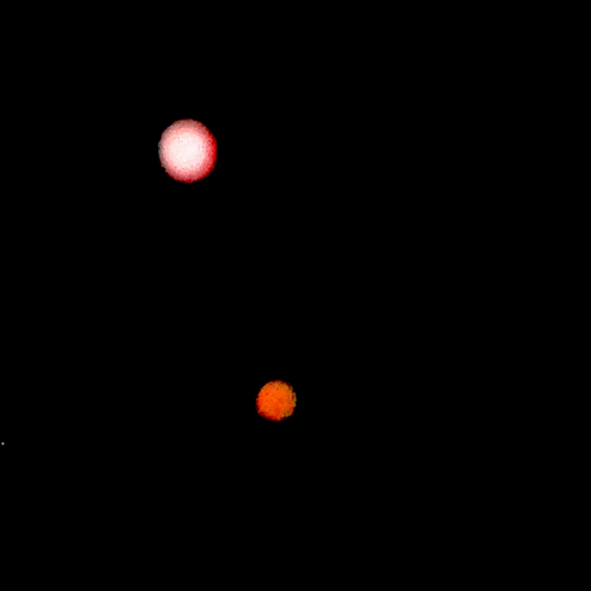
\includegraphics[width=.50\linewidth]{Image.png}

Note that this will not put an figure environment in LaTeX
files, so the image won't float this way. For this to
achieve to have to put \%image, \%img or \%figure before the
line. You don't need the extention then.

\begin{figure}[hbt]
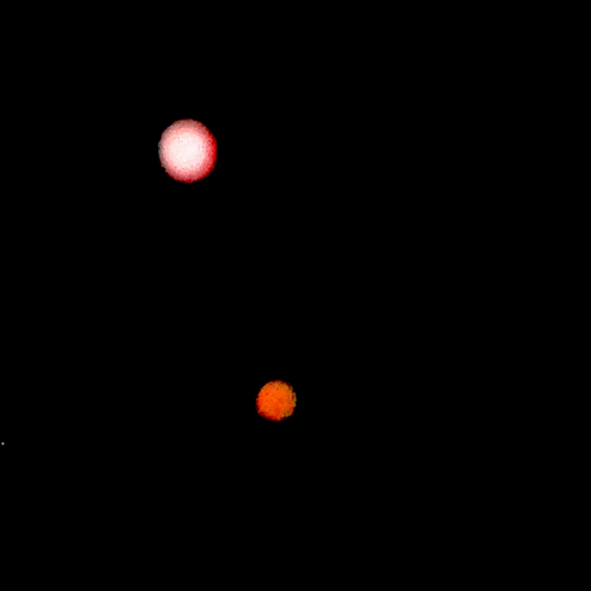
\includegraphics[height=.20\textheight]{Image}
\caption{Mars und Mond}
\end{figure}


\end{document}

%%% Local Variables:
%%% mode: latex
%%% TeX-master: t
%%% End:
